\documentclass[11pt,a4paper,landscape]{article}

\usepackage{main}
\usepackage{cours}

\usepackage{array}

\newcolumntype{C}[1]{>{\centering\arraybackslash}m{#1}}

\renewcommand{\typedocument}{Fiche}
\renewcommand{\classe}{3e}
\renewcommand{\titre}{Formules}

\begin{document}

\renewcommand{\arraystretch}{2}

\setlength{\tabcolsep}{4pt}

\begin{tabular}{|C{5cm}|C{9cm}|C{3.5cm}|C{10cm}|}
\hline
\rowcolor{gray!30}
{\normalsize\color{black}\textbf{Formule}} &
{\normalsize\textbf{Grandeurs et unités}} &
{\normalsize\textbf{Triangle}} &
{\normalsize\textbf{Autres formules}}\\ \hline
\huge$\rho = \frac{m}{V}$ 
    & \begin{itemize}
        \item $\rho$ : \textbf{masse volumique} (kg/m$^3$ ou g/cm$^3$)
        \item $m$ : \textbf{masse} (kg ou g)
        \item $V$ : \textbf{volume} (m$^3$ ou cm$^3$)
    \end{itemize}
    & 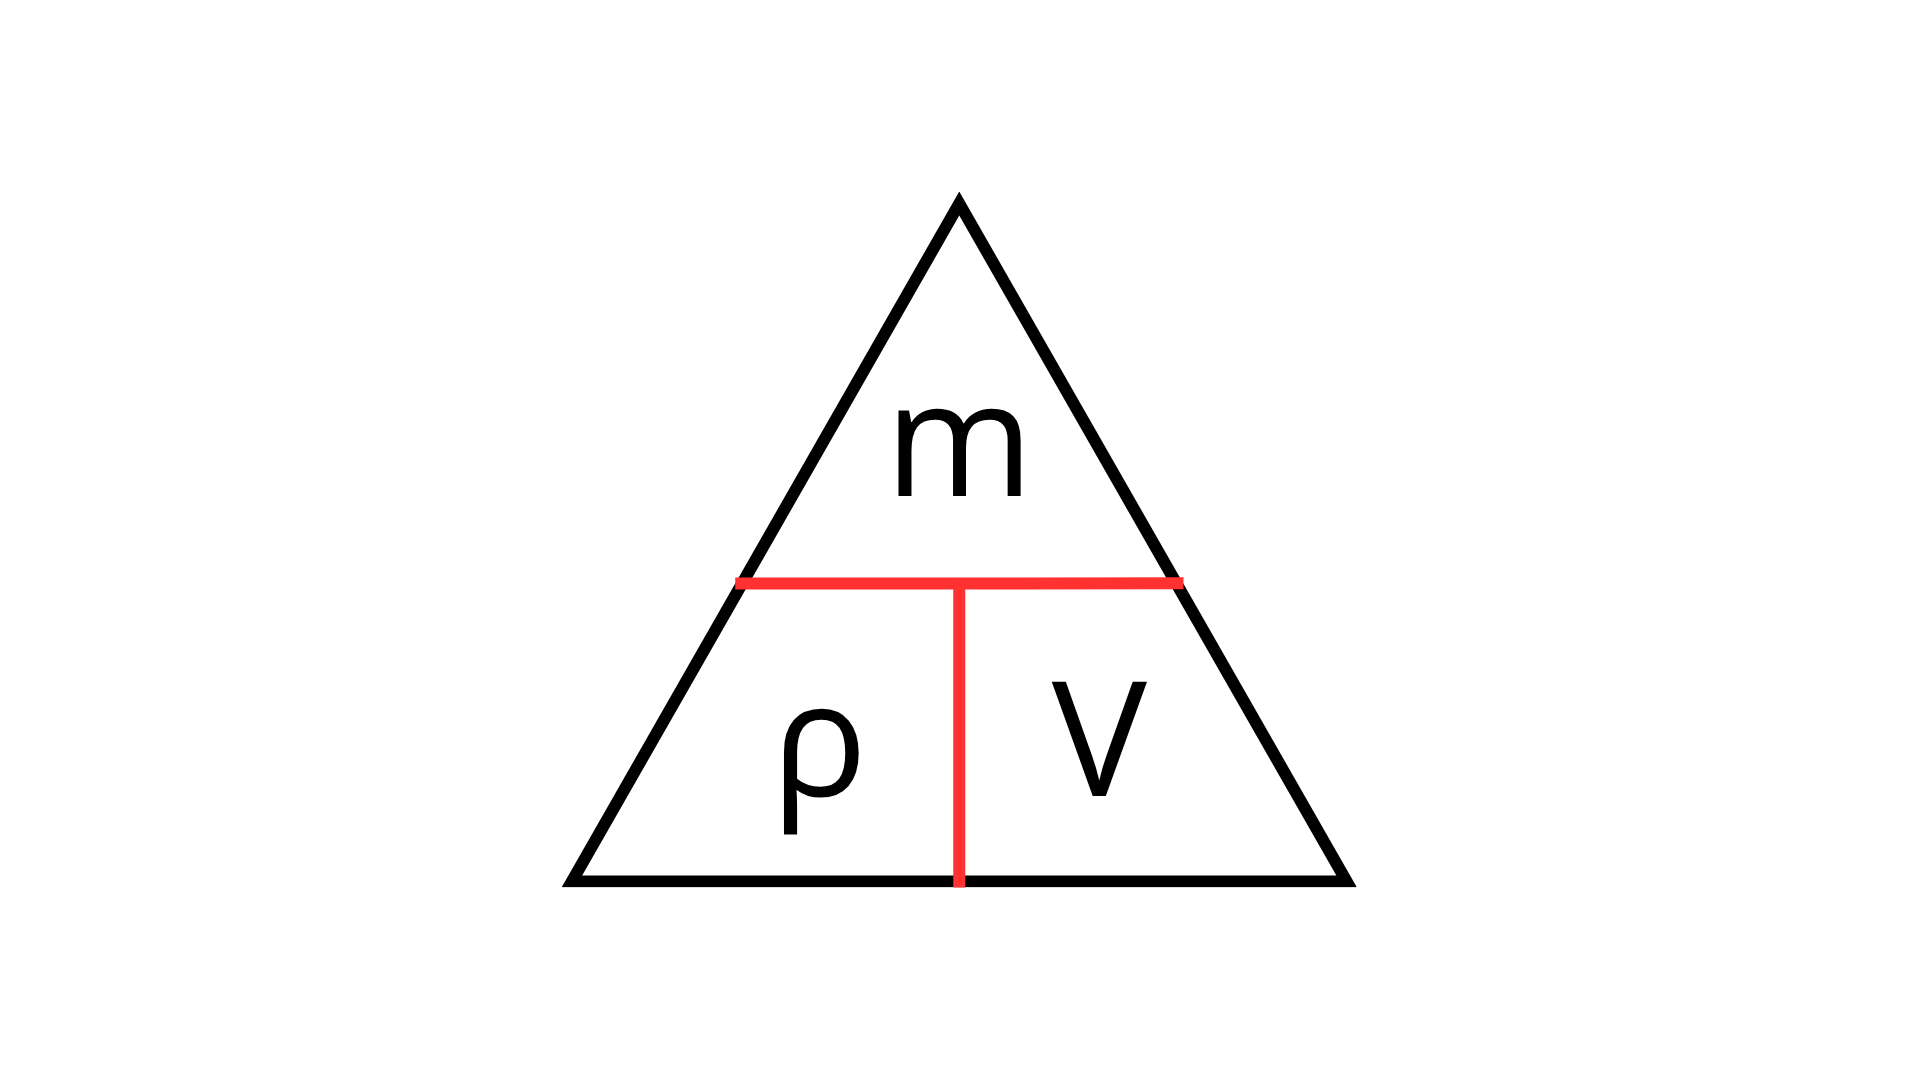
\includegraphics[width=2.6cm]{images/masse volumique.png}
    & $m = \rho \times V$, \hspace{1cm} $V = \frac{m}{\rho}$
\\ \hline
\huge$v = \frac{d}{t}$ 
    & \begin{itemize}
        \item $v$ : \textbf{vitesse}  (m/s ou km/h)
        \item $d$ : \textbf{distance} (m ou km)
        \item $t$ : \textbf{temps} (s ou h)
    \end{itemize}
    & 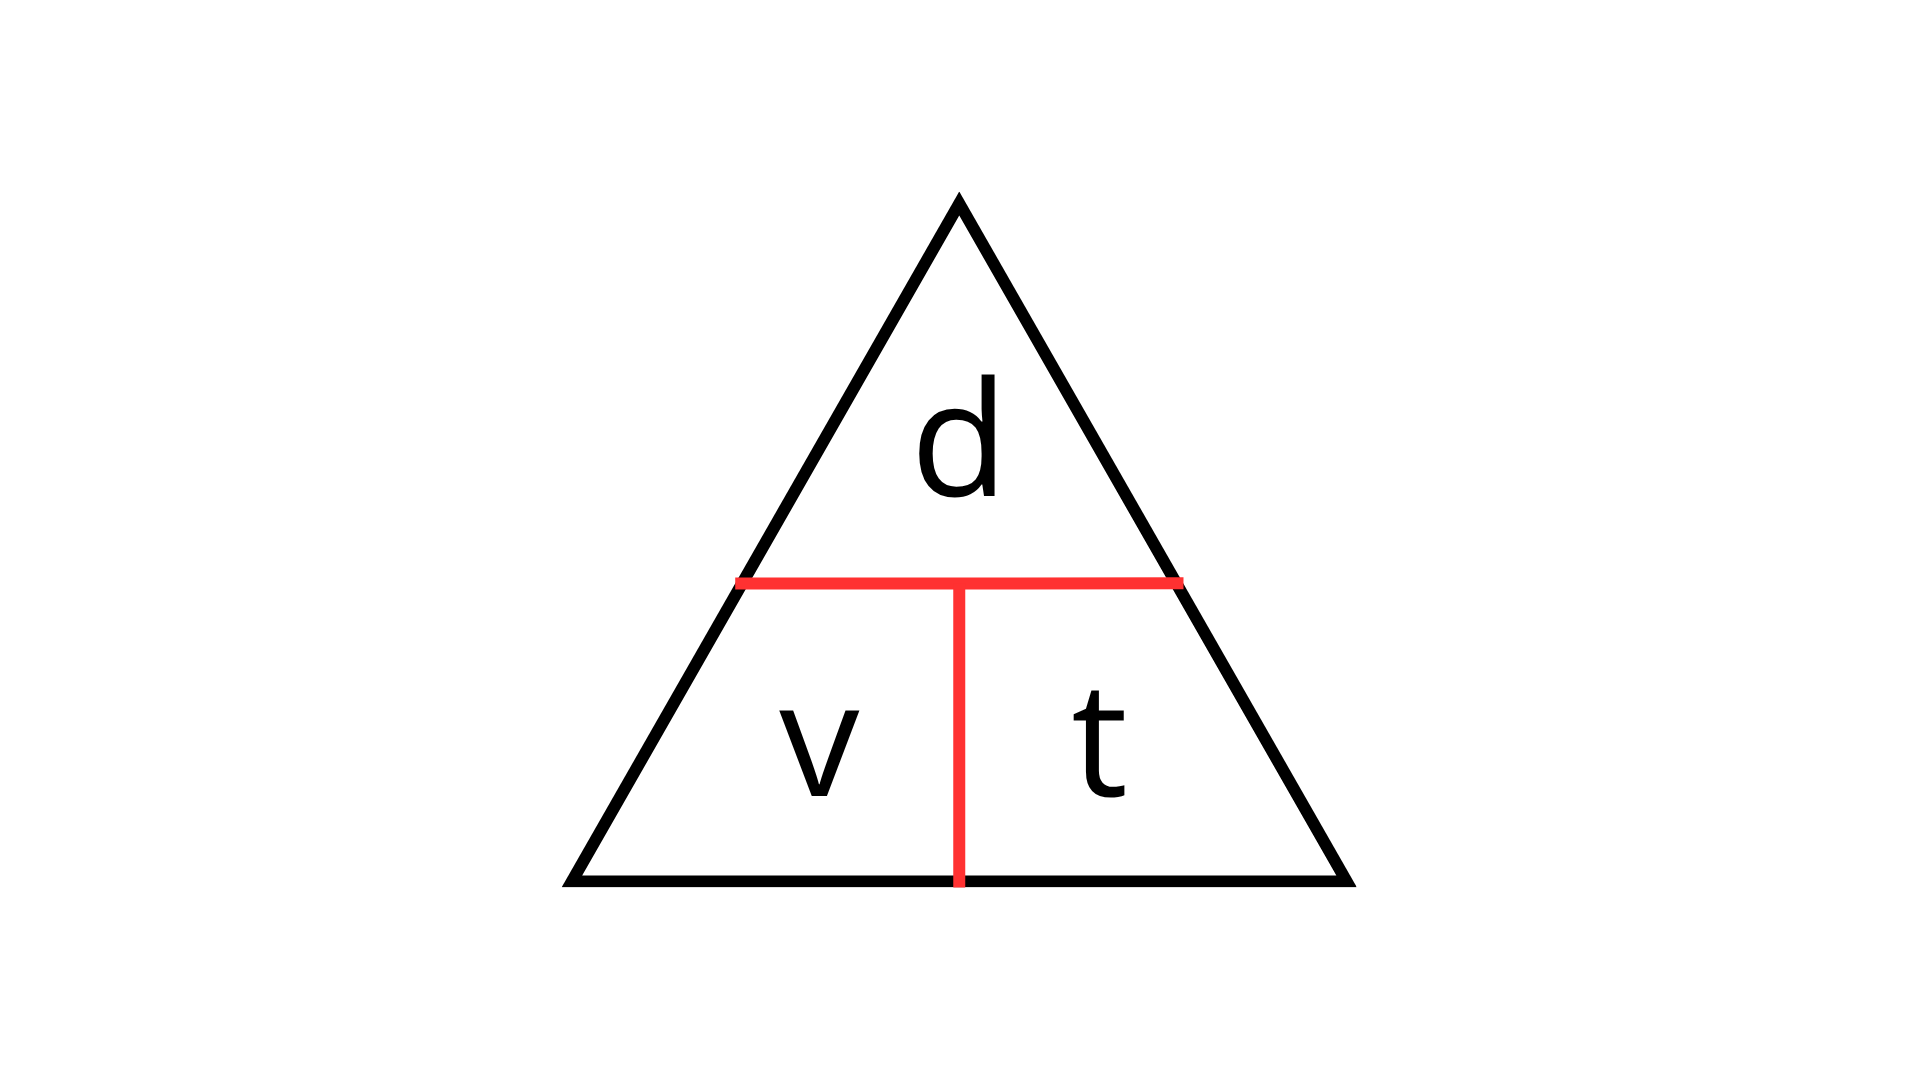
\includegraphics[width=2.6cm]{images/vitesse.png}
    & $d = v \times t$, \hspace{1cm} $t = \frac{d}{v}$
\\ \hline
\LARGE$P = m \times g$ 
    & \begin{itemize}
        \item $P$ : \textbf{poids} (N)
        \item $m$ : \textbf{masse} (kg)
        \item $g$ : \textbf{intensité de la pesanteur} (N/kg)
    \end{itemize}
    & 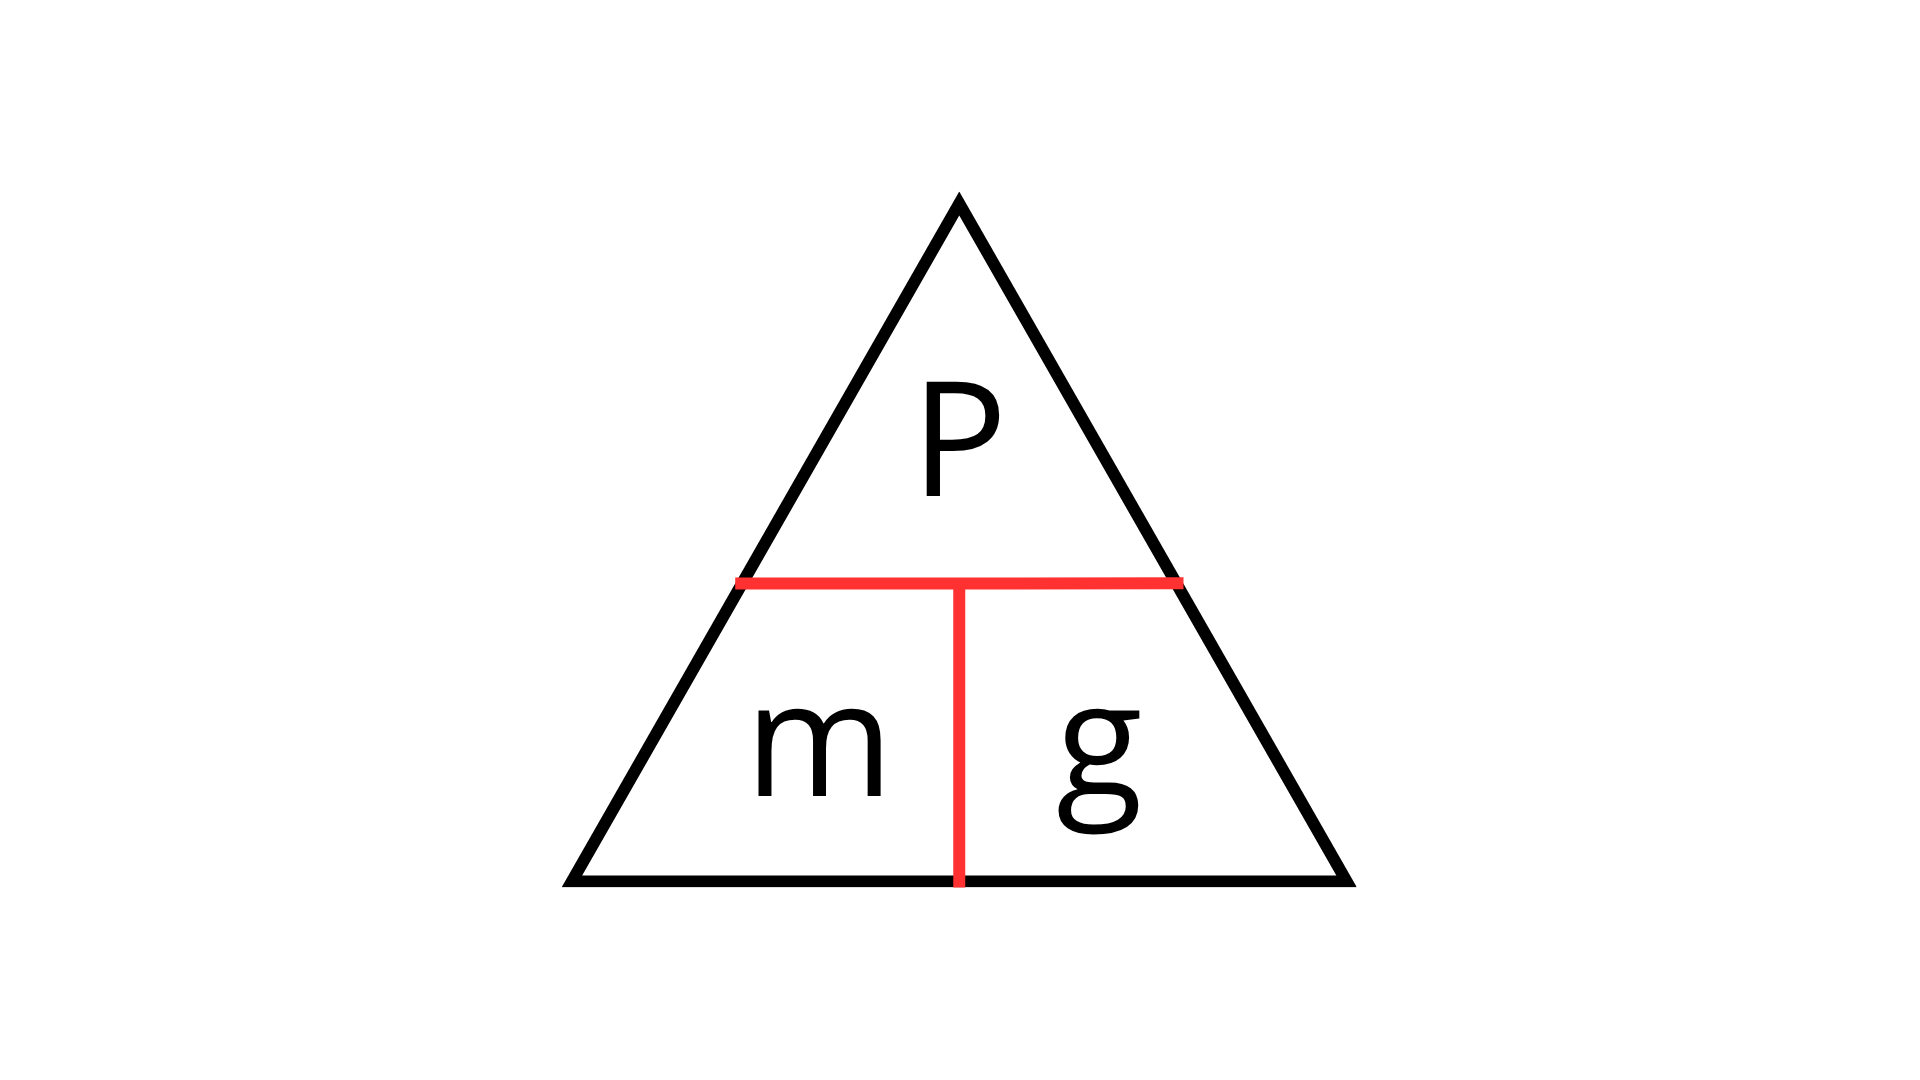
\includegraphics[width=2.6cm]{images/poids.png}
    & $m = \frac{P}{g}$, \hspace{1cm} $g = \frac{P}{m}$
\\ \hline
\LARGE$U = R \times I$ 
    & \begin{itemize}
        \item $U$ : \textbf{tension} (V)
        \item $R$ : \textbf{résistance} (ohm ou $\Omega$)
        \item $I$ : \textbf{intensité} (A)
    \end{itemize}
    & 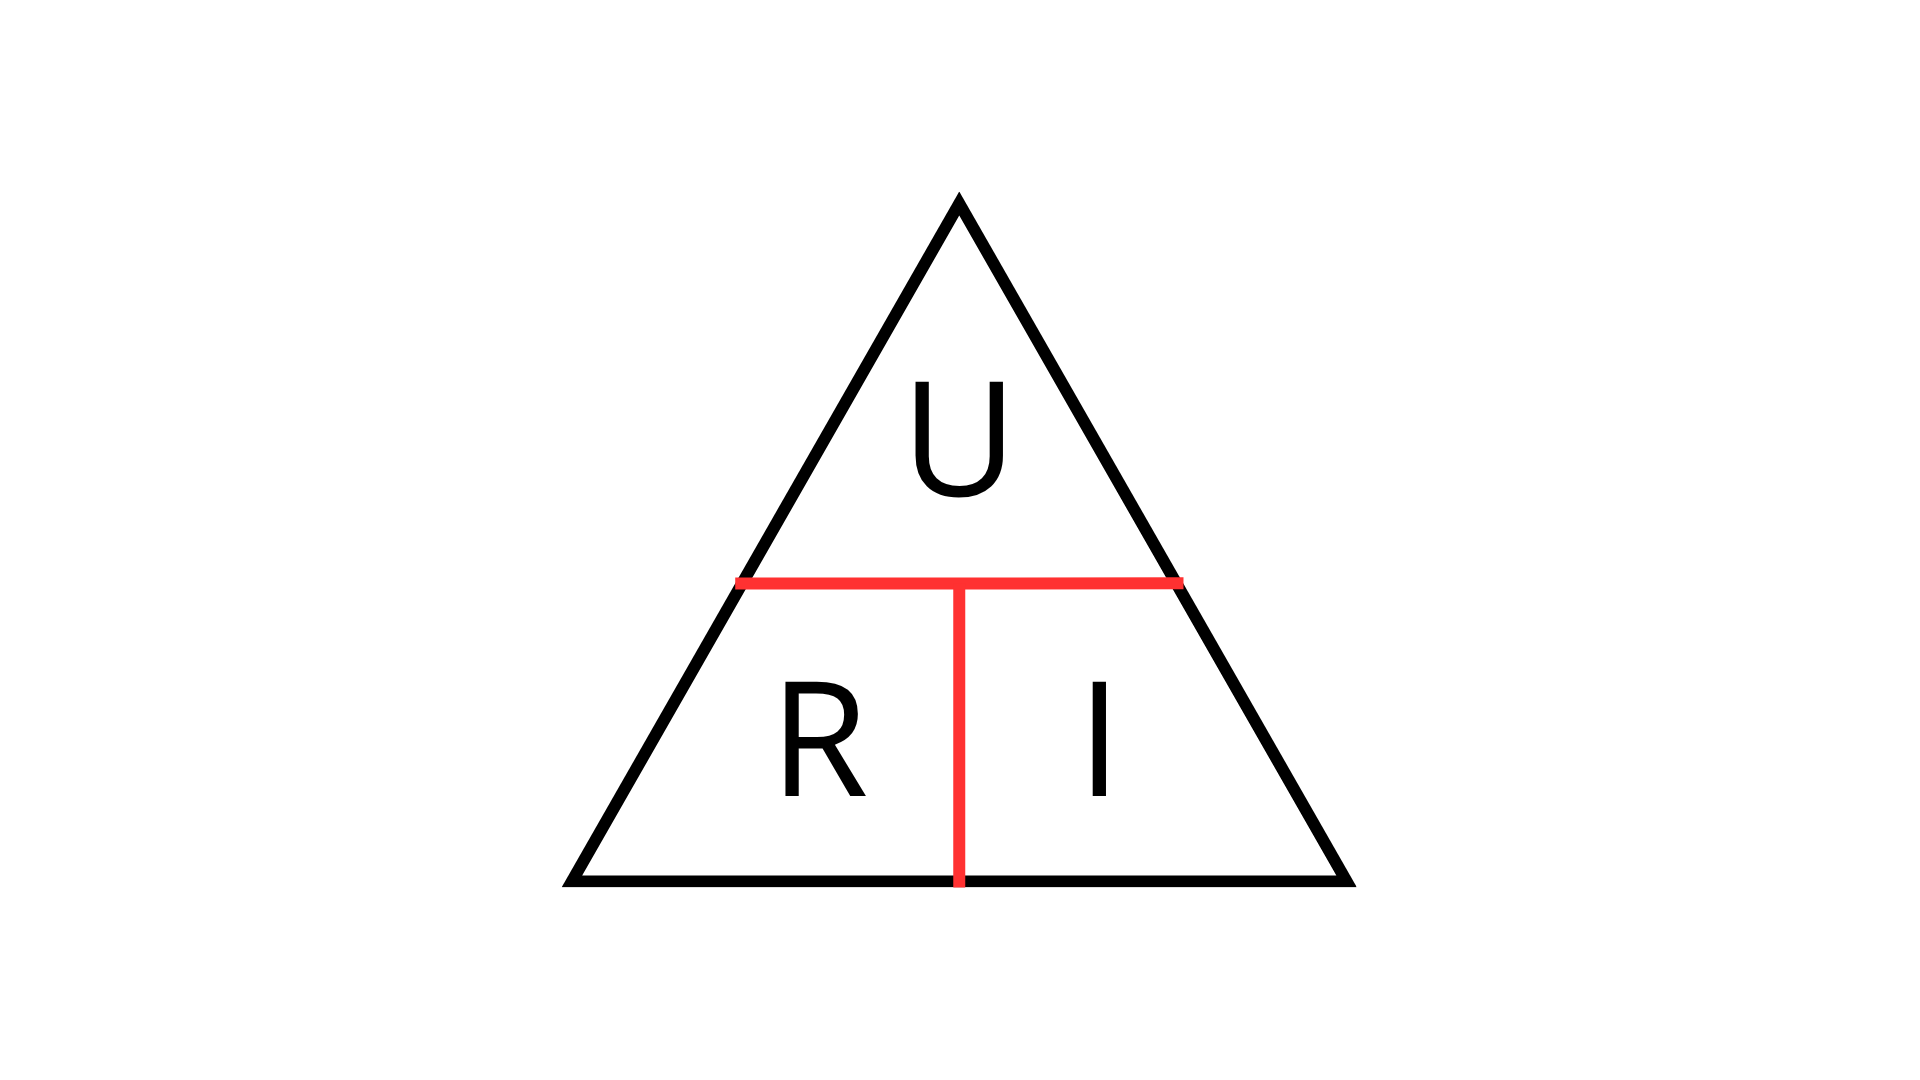
\includegraphics[width=2.6cm]{images/loi ohm.png}
    & $R = \frac{U}{I}$, \hspace{1cm} $I = \frac{U}{R}$
\\ \hline
\LARGE$\mathcal{P} = U \times I$ 
    & \begin{itemize}
        \item $\mathcal{P}$ : \textbf{puissance} (W)
        \item $U$ : \textbf{tension} (V)
        \item $I$ : \textbf{intensité} (A)
    \end{itemize}
    & 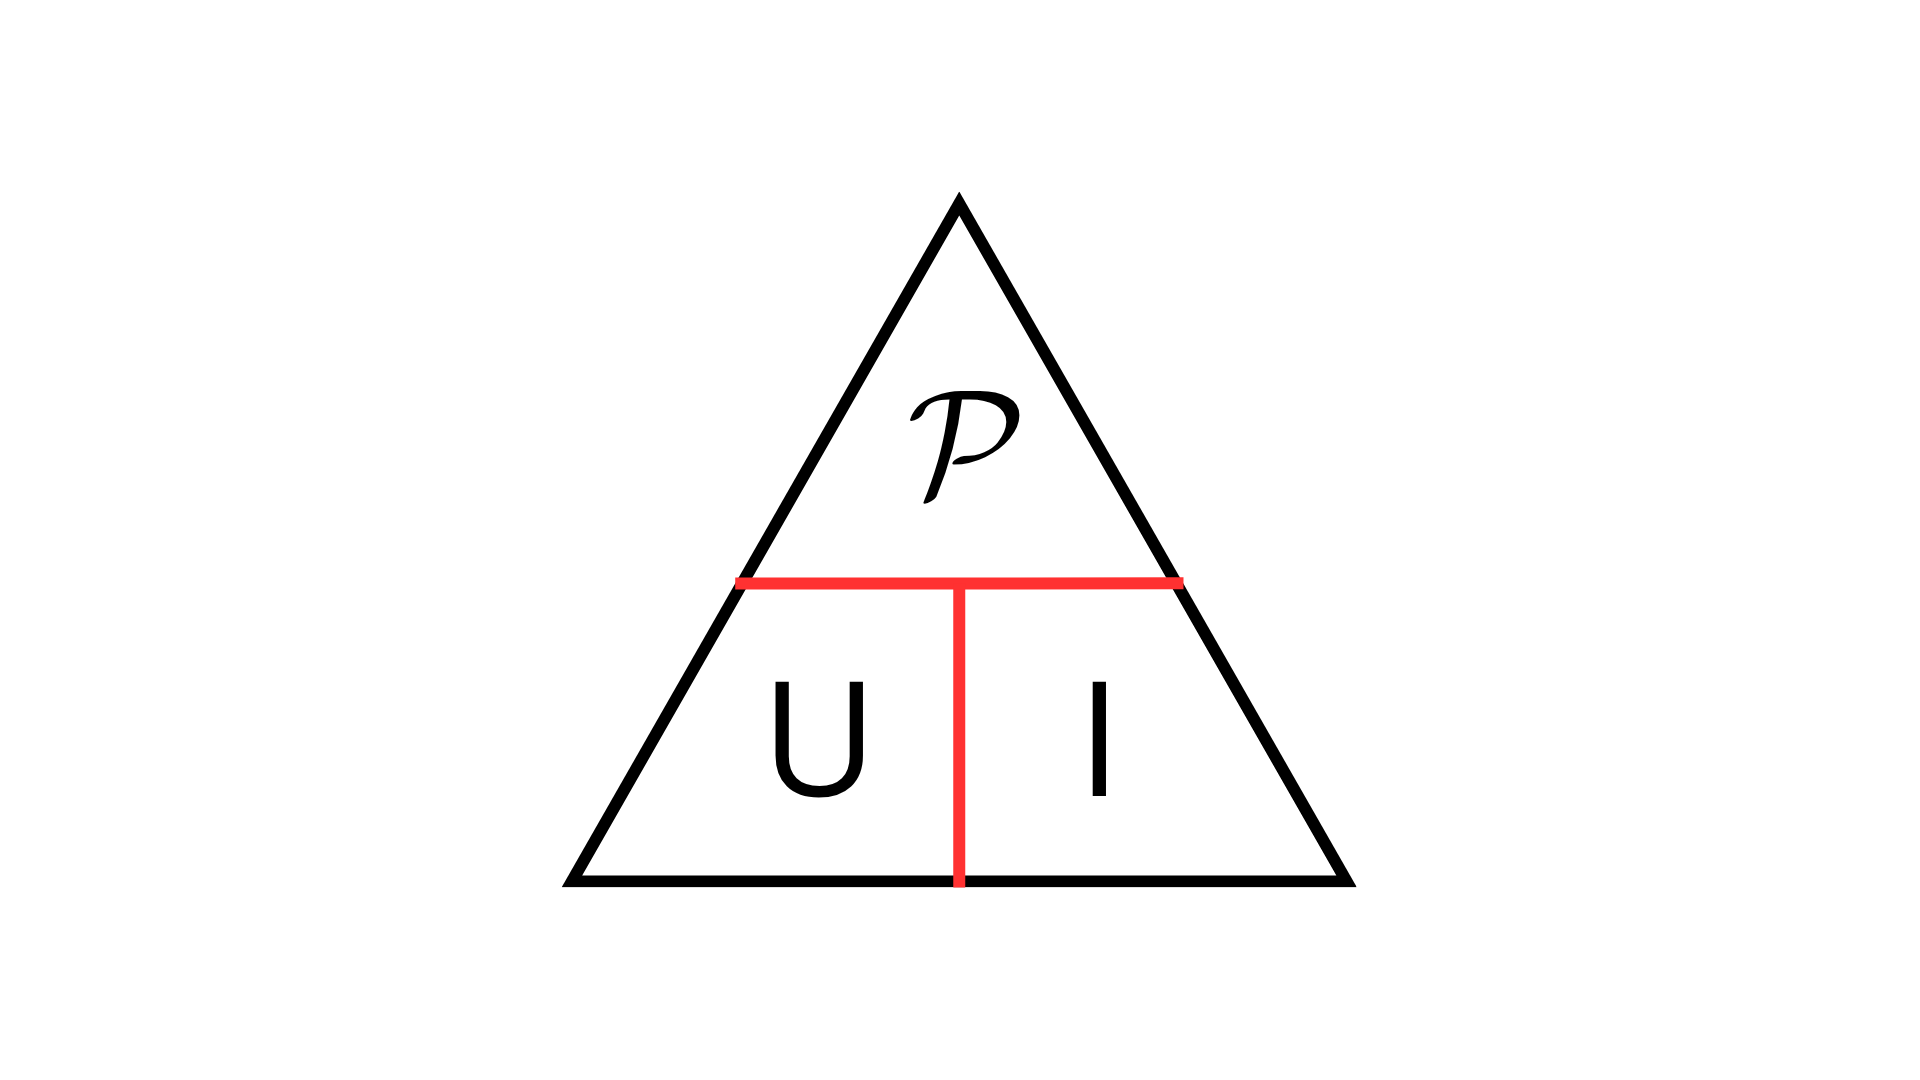
\includegraphics[width=2.6cm]{images/puissance elec.png}
    & $U = \frac{\mathcal{P}}{I}$, \hspace{1cm} $I = \frac{\mathcal{P}}{U}$
\\ \hline
\LARGE$E = \mathcal{P} \times t$ 
    & \begin{itemize}
        \item $E$ : \textbf{énergie} (J ou Wh)
        \item $\mathcal{P}$ : \textbf{puissance} (W)
        \item $t$ : \textbf{temps} (s ou h)
    \end{itemize}
    & 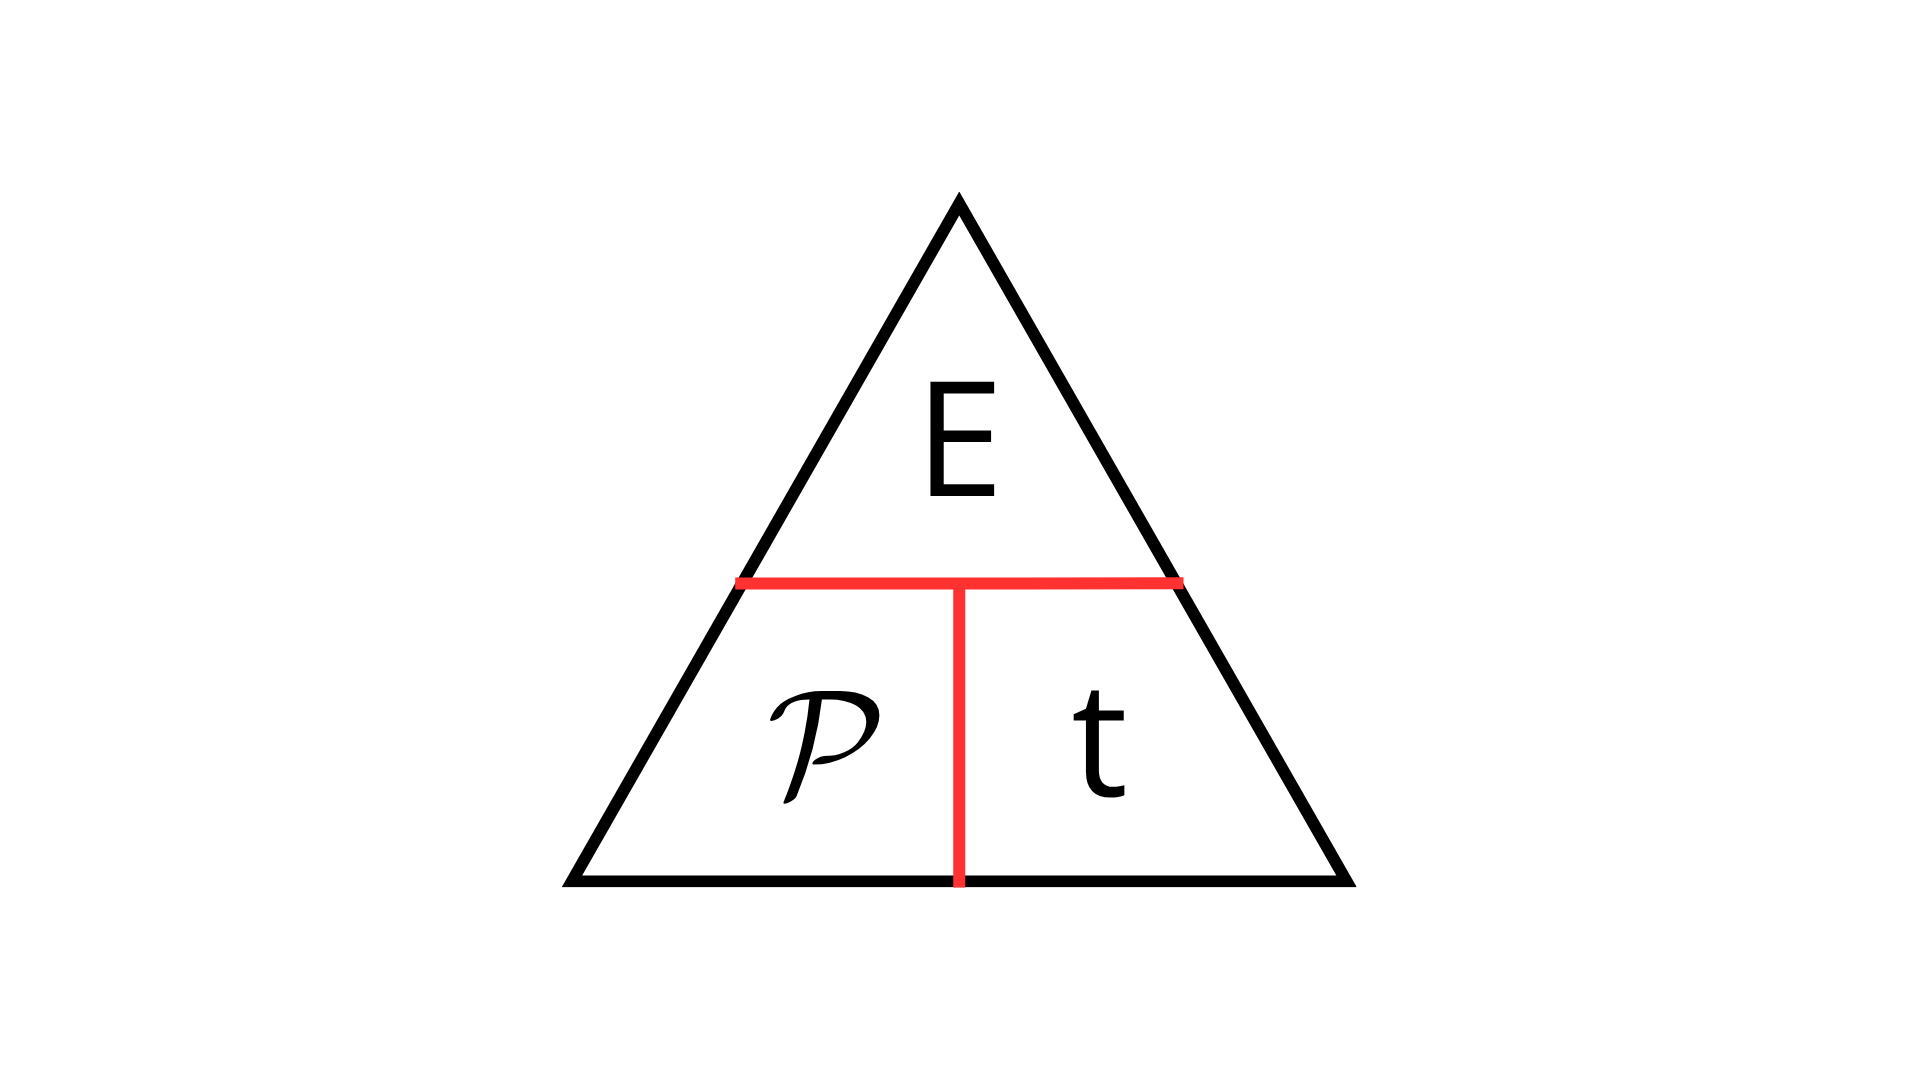
\includegraphics[width=2.6cm]{images/énergie.png}
    & $\mathcal{P} = \frac{E}{t}$, \hspace{1cm} $t = \frac{E}{\mathcal{P}}$
\\ \hline
\LARGE$E_p = m \times g \times h$ 
    & \begin{itemize}
        \item $E_p$ : \textbf{énergie potentielle} (J)
        \item $m$ : \textbf{masse} (kg)
        \item $g$ : \textbf{intensité de la pesanteur} (N/kg)
        \item $h$ : \textbf{hauteur} (m)
    \end{itemize}
    & &
\\ \hline
\LARGE$E_c = \frac{1}{2} \times m \times v^2$ 
    & \begin{itemize}
        \item $E_c$ : \textbf{énergie cinétique} (J)
        \item $m$ : \textbf{masse} (kg)
        \item $v$ : \textbf{vitesse} (m/s)
    \end{itemize}
    & &
\\ \hline
\end{tabular}

\textbf{Pour utiliser le triangle : cacher la grandeur recherchée, ce qui reste indique l'opération à effectuer.}

\end{document}